\documentclass[
        handout,
        %draft,
        ]{beamer}
\usepackage{amssymb,latexsym,amssymb,amsmath,amsbsy,amsopn,amstext,upgreek}
\usepackage{color,multicol}
\usepackage{graphicx,wrapfig,fancybox,watermark,graphics}
\usepackage{picins}
%\usepackage{emp}
%\usepackage{pstricks,pst-plot}
\usepackage{pgf}
\usepackage{movie15}
\usepackage{hyperref}
\usepackage{pdfpages}
\usepackage{listings,bera}
\definecolor{keywords}{RGB}{255,0,90}
\definecolor{comments}{RGB}{60,179,113}
\lstset{language=C,
keywordstyle=\color{keywords},
commentstyle=\color{comments}\emph}
\hypersetup{
    pdfpagemode=FullScreen, % show in full screen?
}
\usepackage{algorithm}
\usepackage{algorithmic}
\renewcommand{\algorithmicrequire}{\textbf{Input:}}
\renewcommand{\algorithmicensure}{\textbf{Output:}}
% reference entry
\usepackage{bibentry, natbib}
% reference style
\bibliographystyle{IEEEtran} 
%reference lib
\nobibliography{refs}

\usepackage[
	%compress,
	minimal,
	%nonav,
	red,
	%gold,
	%numbers,
	%nologo,
	polyu,
	]{beamerthemeHongKong}
\usefonttheme[professionalfonts]{serif}

\title[Tutorial 11]{Tutorial 11: Assignment 5}
\author[COMP210]{Qu Xiaofeng\texorpdfstring{, Teaching Asistant\\\tiny{quxiaofeng.at.polyu@gmail.com, PQ702}}{}}
\institute{COMP210\\Discrete Structure}
\date{\today}

\begin{document}

\frame{\titlepage}

\section*{Table of Contents}

    \begin{frame}{\secname}
        \tableofcontents
    \end{frame}

\AtBeginSubsection[] {
    \begin{frame}<handout:0>{Outline}
        \tableofcontents[current,currentsubsection]
    \end{frame}
}

\section[Review]{Review of Probability}
    \begin{frame}[c,shrink]{\secname}
        \label{review}
        \centerline{\includegraphics[height=0.85\textheight,page=2]{tut_probability}}
    \end{frame}
    
    \begin{frame}[c,shrink]{\secname\ cont.}
        \centerline{\includegraphics[height=0.85\textheight,page=3]{tut_probability}}
    \end{frame}
    
    \begin{frame}[c,shrink]{\secname\ cont.}
        \centerline{\includegraphics[height=0.85\textheight,page=4]{tut_probability}}
    \end{frame}
    
    
    
\section{Problems}
    \subsection{Problem 1}    
        \begin{frame}[c]{\subsecname}
            \emph{In how many ways can five distinct Martians and five distinct Jovians be seated at circular table?}\\$\;$\\\pause
            The answer is 9!=36288. \qed
        \end{frame}



    \subsection{Problem 3}
        \begin{frame}[c]{\subsecname}
            \emph{Find the number of integer solutions of $x_1 + x_2 + x_3 = 15$ subject to $ x_1, x_2, x_3 \geq 0$.}\\$\;$\\\pause
            The answer is C(15+3-1,15)=136. \qed
        \end{frame}



    \subsection{Problem 7.1}
        \begin{frame}[c]{\subsecname}
            \emph{Four microprocessors are randomly selected from 100 microprocessors among which 10 are defective. Find the probability of obtaining no defective microprocessors?} \\$\;$\\ \pause
            The answer is C(90,4)/C(100,4)=0.6516. \qed
        \end{frame}



    \subsection{Problem 8.1}
        \begin{frame}[c]{\subsecname}
            \emph{Consider three persons who each randomly choose a locker among 12 consecutive
lockers. What is the probability that the three lockers chosen are consecutive.}\\$\;$\\\pause
            The answer is 10/C(12,3)=1/22. \qed
        \end{frame}


\section{Problems cont.}
    \subsection{Problem 11.1}
        \begin{frame}[c]{\subsecname}
            \begin{columns}
            \column{0.75\textwidth}
                \emph{State which graphs are bipartite graphs. If the graph is bipartite, specify the disjoint vertex sets}\\$\;$\\
                \uncover<2->{The answer is Bipartite. $V_1=\{v_1,v_2,v_5\},\; V_2=\{v_3,v_4\}$. \qed}
            \column{28.6mm}
                \begin{figure}
                    \centering
                    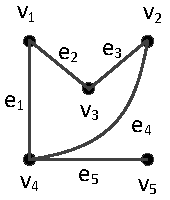
\includegraphics[width=28.6mm]{tut11p10}
                \end{figure}
            \end{columns}
        \end{frame}
        
        

    \subsection{Problem 14.1}
        \begin{frame}[c]{\subsecname}
            \begin{columns}
            \column{0.75\textwidth}
                \emph{Consider the graph in the figure. Find the degree for each vertex in the graph}\\$\;$\\
                \uncover<2->{The answer is that every vertex has degree 4. \qed}
            \column{34mm}
                \begin{figure}
                    \centering
                    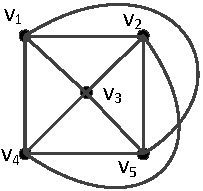
\includegraphics[width=34mm]{tut11p13_1}
                \end{figure}
            \end{columns}
        \end{frame}



%    \subsection{Problem 15}
%        \begin{frame}[c]{\subsecname}
%            \emph{Show that the maximum number of edges in a simple, bipartite graph with n
%vertices is (n-1)(n-2)/2.}\\$\;$\\\pause
%            Let $G$ be a simple, disconnected graph with $n$ vertices having the maximum number of edges. Show that G has two components. If one component has $i$ vertices, show that the components are $K_i$ and $K_{n-i}$. Use Excercise 11, Section 8.1, to find a formula for the number of edges in $G$ as a function of $i$. Show that the maximum occurs when $i=1$. \qed
%        \end{frame}
%
%
%
%    \subsection{Problem 19.1}
%        \begin{frame}[c]{\subsecname}
%            \begin{figure}
%                \centering
%                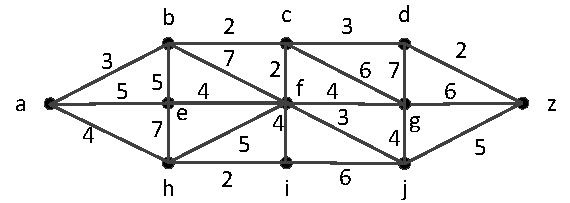
\includegraphics[width=96.3mm]{tut11p17_1}
%            \end{figure}
%            \emph{Find the length of a shortest path and a shortest path between each pair of
%vertices in the weighted graph. 1) a,f.}\\$\;$\\\pause
%            The answer is 7;(a, b, c, f). \qed
%        \end{frame}
%
%
%\section{Problems cont.}
%    \subsection{Problem 21}
%        \begin{frame}[c]{\subsecname}
%            \emph{Show that a tree is a bipartite graph.}\\$\;$\\\pause
%            Let $T$ be a tree. Root $T$ at some arbitrary vertex. Let $V$ be the set of vertices on even levels and let $W$ be the set of vertices on odd levels. Since each edge is incident on a vertex in $V$ and a vertex in $W$, $T$ is a bipartite graph.\qed
%        \end{frame}
%
%
%
%    \subsection{Problem 23}
%        \begin{frame}[c]{\subsecname}
%            \emph{Show that a graph $G$ with $n$ vertices and fewer than $n-1$ edges is not connected.}\\$\;$\\\pause
%            Suppose that $G$ is connected. Add parallel edges until the resulting graph $G^*$ has $n-1$ edges. Since $G^*$ is connected and has $n-1$ edges, by Theorem 9.2.3, $G^*$ is acyclic. But adding an edge in parallel introduces a cycle. Contradiction. \qed
%        \end{frame}
%
%
%
%    \subsection{Problem 26.1}
%        \begin{frame}[c]{\subsecname}
%            \emph{Find a spanning tree for each graph using depth-first and breadth-first search.}\\
%            \begin{figure}
%                \centering
%                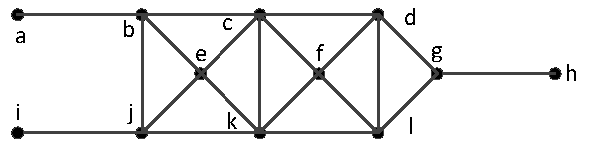
\includegraphics[width=99.6mm]{tut11p23_1_1}
%            \end{figure}\pause
%            \begin{figure}
%                \centering
%                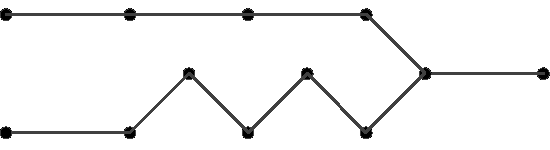
\includegraphics[width=93mm]{tut11p23_1_2} \qed
%            \end{figure}
%        \end{frame}
%
%
%
%    \subsection{Problem 27}
%        \begin{frame}[c]{\subsecname}
%            \emph{Let $T$ and $T^\prime$ be two spanning trees of a connected graph $G$. Suppose that an edge $x$ is in $T$ but not in $T^\prime$. Show that there is an edge $y$ in $T^\prime$ but not in $T$ such that $( T - \{ x \} ) \cup \{ y \} $ and $(T^\prime - \{ y \} ) \cup \{ x \} $ are spanning trees of $G$.}\\$\;$\\\pause
%            Suppose that $x$ is incident on vertices $a$ and $b$. Removing $x$ form $T$ produces a disconnected graph with two components, $U$ and $V$. Vertices $a$ and $b$ belong to different components\--- say, $a \in U$ and $b \in V$. There is a path $P$ from $a$ to $b$ in $T^\prime$. As we move along $P$, at some point we encounter an edge $y=(v,w)$ with $v \in U$, $w \in V$. Since adding $y$ to $T-\{x\}$ produces a connected graph, $(T-\{x\}) \cup \{y\}$ is a spanning tree. Clearly, $(T^\prime-\{y\}) \cup \{x\}$ is a spanning tree. \qed
%        \end{frame}
    

        
        

    \subsection{Homework Reminder}
        \begin{frame}<handout:0>[c]{\subsecname}
            \begin{itemize}[<+-|alert@+>]
            	\item Hardcopy is preferred. If you want to upload scanned softcopy to webct, make sure write Student ID on scanned paper. The multi-page pdf is best choice of the scaning format.
            	\item Answers are expected to be in increasing order. If not, please mark very clearly.
            	\item Check the problems carefully, especially the questions. Sometimes you have to prove your answer or draw the graph.
            \end{itemize}
        \end{frame}
    
    \begin{frame}<handout:0>[c]{\secname}
        \centerline{\Large{Any questions?}}
    \end{frame}
    
    
    
\end{document}



